%%%%%%%%%%%%%%%%%%%%%%%%%%%%%%%%%%%%%%%%%%%%%%%%%%%%%%%%%%%%%%%%%%%%%%%%
\chapter{Related Work}
\label{sec:relatedWork}
%%%%%%%%%%%%%%%%%%%%%%%%%%%%%%%%%%%%%%%%%%%%%%%%%%%%%%%%%%%%%%%%%%%%%%%%

Most of the works published in the field of streamline placement algorithms can be divided into two categories:
\subsection{Image-Guided}
The goal of this approach is to achieve a very uniform, almost "hand-drawn" appearance.
Generated images will usually have high visual quality, at the risk of potentially missing or misrepresenting important features.
\\\\
One of the first and most prominent examples in this category was written by Greg Turk and David Banks~\cite{TurkBanks}.
In their research paper, a function (called the "Energy Function") is defined such that it maps an input image containing the potential streamlines to a scalar.
The scalar represents the quality of the image, roughly defined as the uniformity of the gray scales it contains. 
Adding/moving/removing/resizing streamlines is done randomly, at every step the energy function is used to determine whether the change gets accepted or discarded.
The algorithm is finished when the energy function reaches a minimal threshold, or a maximum number of consecutive rejected steps is exceeded.

This algorithm will also serve as the basis for this thesis, with subsequent extensions for time coherence being added.

\subsection{Feature-Guided}
Feature-Guided algorithms examine the underlying field structure before placing seeds.
They search for critical points or patterns in the field and then seed around them, capturing them in much higher detail.
The resulting images inherently represent the critical points much better, at the cost of some visual appeal compared to the aforementioned group.
\bigskip

\begin{center}
    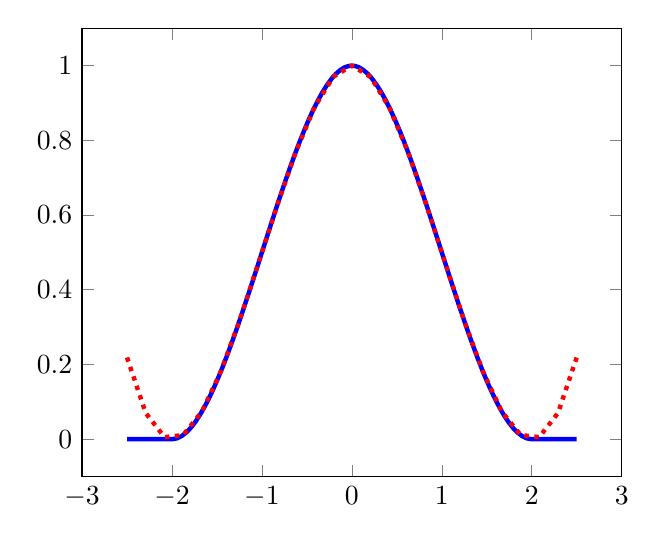
\begin{tikzpicture}
    \def\r(#1){abs(#1) / 2}%
    \begin{axis}
        \addplot[color=blue, ultra thick, samples=100, domain=-2.5:2.5]{
            \r(x) < 1 ? 2*(\r(x))^3-3*(\r(x))^2+1 : 0
        };
        \addplot[color=red, dotted, ultra thick, domain=-2.5:2.5]{
            2*(\r(x))^3-3*(\r(x))^2+1
        };
    \end{axis}
\end{tikzpicture}
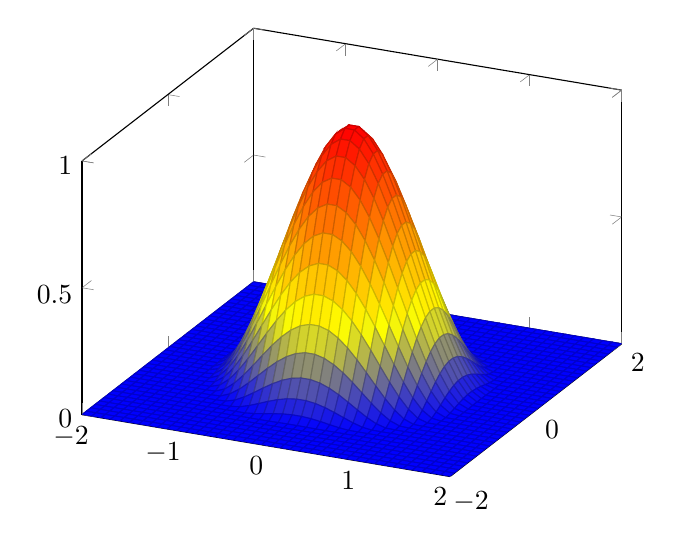
\begin{tikzpicture}[]
    \def\r(#1,#2){(((#1)^2 + (#2)^2) / 2)^0.5}%
    \def\K(#1,#2){2 * \r(#1,#2)^3 - 3 * \r(#1,#2)^2 + 1}
    \begin{axis}[
        % xmin=-2.5,xmax=2,
        % ymin=-2.5,ymax=2,
        zmin= 0  ,zmax=1,
        % axis line style={draw=none},
        % axis equal image,
    ]
    \addplot3[
        surf,
        domain=-2:2,
        samples=40
    ]
    % K(x,y) = 2r^3 - 3r^2 + 1 if r < 1 else 0
    % r = sqrt(x^2 + y^2) / R
    % R = desired radius, lets use 2
    % therefore we get:
    % r = sqrt(x^2 + y^2) / 2
    % K(x,y) = sqrt(x^2 + y^2) / 2 < 1 ? 2 * (sqrt(x^2 + y^2) / 2) ^ 3 - 3 * (sqrt(x^2 + y^2) / 2) ^ 2 + 1 : 0
    {\r(x,y) < 1 ? \K(x,y) : 0};% < 1 ? 2 * r(x,y) ^ 3 - 3 * r(x,y) ^ 2 + 1 : 0};
    \end{axis}
\end{tikzpicture}

\end{center}


\subsection{Other Relevant Works}
\begin{itemize}
    \item \href{https://www.cs.purdue.edu/homes/xmt/papers/Coherent-Streamline_Tsinghua_2012.pdf}{Time Coherence in 2D}
    \item \href{https://www.cg.tuwien.ac.at/courses/Visualisierung1/2015W/exercises/Streamlines_Jobard&Lefer.pdf}{Approach I've used so far due to simplicity}
\end{itemize}

Do not forget to use references~\cite{Hanser2019energy} like done here~\cite{Hofmann2019dependentVectors} to enable the bibliography~\cite{Jung2017tumble, Sagrista2019GaiaSky, Sdeo2018fullerene, Zheng2019equivalence}.